\documentclass[aspectratio=169,handout]{beamer}
\usepackage{borelian}
\usepackage{multirow}


\begin{document}
    \classtitle{5}{Manejo de datos con Python}{7 de enero de 2026}

    \begin{frame}[fragile]{Antes de \texttt{pandas}: diccionarios}
        El diccionario es una estructura de datos que almacena datos en forma \texttt{llave:valor}. 
        \begin{minted}{python}
            >>> country_capitals = {
            ...    "Germany": "Berlin",
            ...    "Canada": "Ottawa",
            ...    "England": "London",
            ... }
            >>> country_capitals["Canada"] # Buscamos la capital de Canadá
        \end{minted}
    \end{frame}


    \begin{frame}{¿Cómo trabajaremos los datos?}
        \begin{itemize}
            \item La información puede almacenarse en diferentes formatos: \textbf{grafos}, \textbf{árboles}, \textbf{tablas}, \textbf{diccionarios}, entre otros.
            \item En este curso, nos enfocaremos en datos tabulares (tablas). Este es el formato más simple y utilizado.
            \item El paquete \texttt{pandas} ofrece muchas funciones y estructuras de datos para procesar este formato de datos.
        \end{itemize}
    \end{frame}

    \begin{frame}{Paquete \texttt{pandas} en Python}
        \begin{block}{¿Por qué \texttt{pandas}?}    
            \texttt{pandas} es una librería muy flexible que permite manejar y visualizar datos. 
            \begin{itemize}
                \item Contiene estructuras y herramientas para manejar datos de manera conveniente.
                \item Es mucho mas flexible que otros programas (p. ej., Excel), por lo que nos permite hacer cosas más complicadas y útiles para aplicaciones de inteligencia artificial.
                \item Es capaz de manejar grandes conjuntos de datos, pero existen librerías más sofisticadas como \texttt{dask} o \texttt{polars}.
            \end{itemize}
        \end{block}
    \end{frame}

    \begin{frame}[fragile]{Empezando con \texttt{pandas}}
        Primero importamos el paquete para hacer uso de todas sus funciones.
        \begin{minted}{python}
            >>> import pandas # Importamos el paquete
            >>> data = pandas.read_csv("datos.csv") # Cargamos un CSV
        \end{minted}
        Existe una manera mas conveniente de hacer esto. 
        \begin{minted}{python}
            >>> import pandas as pd
            >>> data = pd.read_csv("datos.csv")
        \end{minted}
        Así, evitamos escribir \mintinline{python}{pandas} en cada llamada a una función. También, comúnmente usaremos la librería \mintinline{python}{numpy} en conjunto con pandas.
        \begin{minted}{python}
            >>> import numpy as np
        \end{minted}
    \end{frame}

    \begin{frame}{Estructuras de datos en \texttt{pandas}}
        Usando diccionarios podemos crear nuevas estructuras de datos. Nos enfocaremos en las \emph{series} (\mintinline{python}{pd.Series}) y \emph{data frames} (\mintinline{python}{pd.DataFrame}).
        \begin{table}[H]
            \centering
            \begin{tabular}{c|c|l}
                Dim. & Nombre & Descripción \\
                \hline
                1D & \mintinline{python}{pd.Series} & Arreglo de elementos 1D de un sólo tipo. \\
                2D & \mintinline{python}{pd.DataFrame} & Arreglo 2D con columnas de tipo \mintinline{python}{pd.Series}.
            \end{tabular}
            \caption{Tipos de estructuras de datos en \texttt{pandas}.}
        \end{table}
    \end{frame}

    \begin{frame}[fragile]{Objetos de tipo \mintinline{python}{pd.Series}}
        Un objeto de tipo \mintinline{python}{pd.Series} es un arreglo 1-dimensional que contiene una secuencia de valores del mismo tipo. Este arreglo tiene asociado un arreglo de etiquetas, llamado \emph{index}. 

        \begin{figure}[H]
            \centering
            \includegraphics[width=0.2\linewidth]{days/03/images/series.png}
            \caption{Ejemplo de un objeto de tipo \mintinline{python}{pd.Series}.}
        \end{figure}
    \end{frame}

    \begin{frame}[fragile]{Objetos de tipo \mintinline{python}{pd.Series}}
        \begin{itemize}
            \item Podemos crear un objeto de tipo \mintinline{python}{pd.Series} usando un diccionario. 
        \end{itemize}
        \begin{minted}{python}
            >>> dicc = {"a": 3, "b": 2, "c" :1} 
            >>> obj = pd.Series(dicc)
            >>> obj
        \end{minted}
        Imprime
        \begin{minted}{python}
            a 3
            b 2
            c 1
            dtype: int64
        \end{minted}
    \end{frame}

    \begin{frame}[fragile]{Objetos de tipo \mintinline{python}{pd.Series}}
        \begin{itemize}
            \item Podemos crear un objeto de tipo \mintinline{python}{pd.Series} usando una lista.  
        \end{itemize}
        \begin{minted}{python}
            >>> obj = pd.Series([4, 7, -5, 3])
            >>> obj
        \end{minted}
        Imprime
        \begin{minted}{python}
            0 4
            1 7
            2 -5
            3 3
            dtype: int64
        \end{minted}
    \end{frame}

    \begin{frame}[fragile]{Objetos de tipo \mintinline{python}{pd.DataFrame}}
        Un objeto de tipo \mintinline{python}{pd.DataFrame} representa una tabla rectangular de datos. Esta contiene una colección de columnas, donde cada una puede ser de un tipo diferente.

        \begin{figure}[H]
            \centering
            \includegraphics[width=0.8\linewidth]{days/03/images/dataframes.png}
            \caption{Ejemplo de un objeto de tipo \mintinline{python}{pd.DataFrame}.}
        \end{figure}
    \end{frame}

    \begin{frame}[fragile]{Objetos de tipo \mintinline{python}{pd.DataFrame}}
        \begin{itemize}
            \item Podemos crear un objeto de tipo \mintinline{python}{pd.DataFrame} usando un diccionario donde cada ítem representa una columna. 
        \end{itemize}

        \begin{columns}
            \column{0.6\textwidth}
            \begin{minted}[fontsize=\small]{python}
                >>> data = {
                ...    "Name": ["Alice", "Bob", "Charlie"],
                ...    "Age": [25, 30, 35],
                ...    "City": ["Berlin", "Ottawa", "Londres"]
                ... }
                >>> df = pd.DataFrame(data)
                >>> df
            \end{minted}
            
            \column{0.4\textwidth}
            \begin{figure}[H]
                \centering
                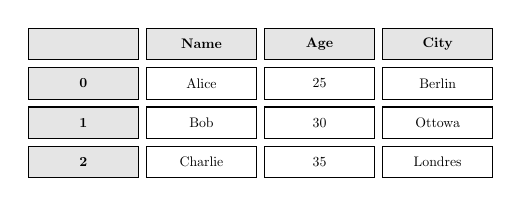
\begin{tikzpicture}[scale=0.5, transform shape,
    cell/.style={
        draw,
        minimum width=2.8cm,
        minimum height=0.8cm,
        align=center
    },
    header/.style={
        cell,
        fill=gray!20,
        font=\bfseries
    }
]

% --- Headers ---
\node[header] (h0) at (0,0) {};
\node[header] (h1) at (3,0) {Name};
\node[header] (h2) at (6,0) {Age};
\node[header] (h3) at (9,0) {City};

% --- Row 0 ---
\node[header] at (0,-1) {0};
\node[cell] at (3,-1) {Alice};
\node[cell] at (6,-1) {25};
\node[cell] at (9,-1) {Berlin};

% --- Row 1 ---
\node[header] at (0,-2) {1};
\node[cell] at (3,-2) {Bob};
\node[cell] at (6,-2) {30};
\node[cell] at (9,-2) {Ottowa};

% --- Row 2 ---
\node[header] at (0,-3) {2};
\node[cell] at (3,-3) {Charlie};
\node[cell] at (6,-3) {35};
\node[cell] at (9,-3) {Londres};

\end{tikzpicture}
            \end{figure}
        \end{columns}
    \end{frame}

    \begin{frame}[fragile]{Básicos de \texttt{pandas}}
        Ahora veremos qué cosas básicas podemos hacer con un \emph{DataFrame}. Volveremos a crear un pequeño conjunto de datos. 
        \begin{minted}{python}
            >>> data = {
            ...    "Name": ["Alice", "Bob", "Charlie", "Kim"],
            ...    "Age": [45, 50, 35, 20],
            ...    "City": ["Berlin", "Ottawa", "Londres", "Hong Kong"]
            ... }
            >>> df = pd.DataFrame(data)
            >>> df
        \end{minted}   
        \begin{figure}[H]
            \centering
            \input{tikz-figures/df_base.tex}
        \end{figure}
    \end{frame}

    \begin{frame}[fragile]{Método \mintinline{python}{head}}
        \begin{itemize}
            \item \mintinline{python}{df.head()} para mirar las primeras filas. Por defecto, se miran $5$, pero podría usarse otro número como argumento (p. ej., \mintinline{python}{df.head(2)}).
        \end{itemize}

        \begin{figure}[H]
            \centering
            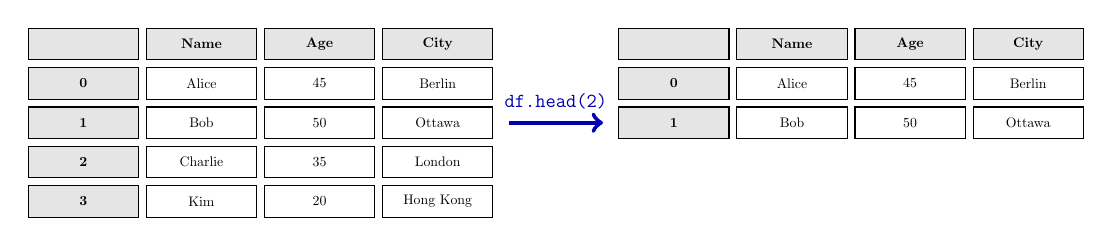
\begin{tikzpicture}[scale=0.5, transform shape,
    cell/.style={
        draw,
        minimum width=2.8cm,
        minimum height=0.8cm,
        align=center
    },
    header/.style={
        cell,
        fill=gray!20,
        font=\bfseries
    }
]

%%%%%%%%%%%%%%%%%%%%%%%%
% DataFrame original
%%%%%%%%%%%%%%%%%%%%%%%%

% --- Headers ---
\node[header] (h0) at (0,0) {};
\node[header] (h1) at (3,0) {Name};
\node[header] (h2) at (6,0) {Age};
\node[header] (h3) at (9,0) {City};

% --- Row 0 ---
\node[header] at (0,-1) {0};
\node[cell] at (3,-1) {Alice};
\node[cell] at (6,-1) {45};
\node[cell] at (9,-1) {Berlin};

% --- Row 1 ---
\node[header] at (0,-2) {1};
\node[cell] at (3,-2) {Bob};
\node[cell] at (6,-2) {50};
\node[cell] at (9,-2) {Ottawa};

% --- Row 2 ---
\node[header] at (0,-3) {2};
\node[cell] at (3,-3) {Charlie};
\node[cell] at (6,-3) {35};
\node[cell] at (9,-3) {London};

% --- Row 3 ---
\node[header] at (0,-4) {3};
\node[cell] at (3,-4) {Kim};
\node[cell] at (6,-4) {20};
\node[cell] at (9,-4) {Hong Kong};

%%%%%%%%%%%%%%%%%%%%%%%%
% Flecha df.head(2)
%%%%%%%%%%%%%%%%%%%%%%%%

\draw[->, ultra thick, blue!70!black]
    (10.8,-2)
    to[out=0,in=180]
    node[midway, above=6pt, font=\ttfamily\Large, text=blue!70!black]
    {df.head(2)}
    (13.2,-2);

%%%%%%%%%%%%%%%%%%%%%%%%
% Resultado df.head(2)
%%%%%%%%%%%%%%%%%%%%%%%%

% --- Headers ---
\node[header] at (15,0) {};
\node[header] at (18,0) {Name};
\node[header] at (21,0) {Age};
\node[header] at (24,0) {City};

% --- Row 0 ---
\node[header] at (15,-1) {0};
\node[cell] at (18,-1) {Alice};
\node[cell] at (21,-1) {45};
\node[cell] at (24,-1) {Berlin};

% --- Row 1 ---
\node[header] at (15,-2) {1};
\node[cell] at (18,-2) {Bob};
\node[cell] at (21,-2) {50};
\node[cell] at (24,-2) {Ottawa};

\end{tikzpicture}

        \end{figure}
    \end{frame}

    \begin{frame}[fragile]{Metodo \mintinline{python}{tail}}
        \begin{itemize}
            \item \mintinline{python}{df.tail()} para mirar las últimas filas. Por defecto, se miran $5$, pero podría usarse otro número como argumento (p. ej., \mintinline{python}{df.tail(2)}).
        \end{itemize}
        \begin{figure}[H]
            \centering
            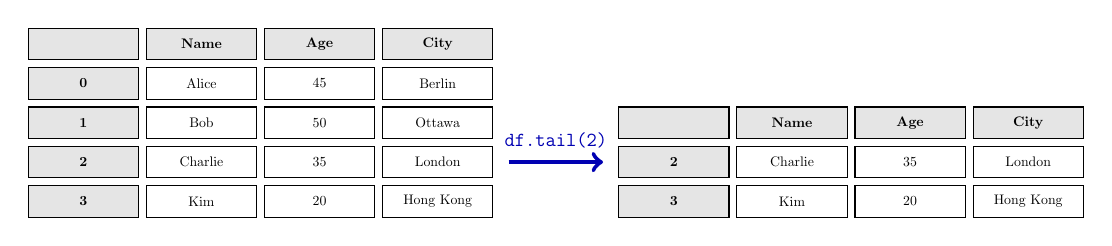
\begin{tikzpicture}[
    scale=0.5, 
    transform shape,
    cell/.style={
        draw,
        minimum width=2.8cm,
        minimum height=0.8cm,
        align=center
    },
    header/.style={
        cell,
        fill=gray!20,
        font=\bfseries
    }
]
    % --- Headers ---
    \node[header] (h0) at (0,0) {};
    \node[header] (h1) at (3,0) {Name};
    \node[header] (h2) at (6,0) {Age};
    \node[header] (h3) at (9,0) {City};

    % --- Row 0 ---
    \node[header] at (0,-1) {0};
    \node[cell] at (3,-1) {Alice};
    \node[cell] at (6,-1) {45};
    \node[cell] at (9,-1) {Berlin};

    % --- Row 1 ---
    \node[header] at (0,-2) {1};
    \node[cell] at (3,-2) {Bob};
    \node[cell] at (6,-2) {50};
    \node[cell] at (9,-2) {Ottawa};

    % --- Row 2 ---
    \node[header] at (0,-3) {2};
    \node[cell] at (3,-3) {Charlie};
    \node[cell] at (6,-3) {35};
    \node[cell] at (9,-3) {London};

    % --- Row 3 ---
    \node[header] at (0,-4) {3};
    \node[cell] at (3,-4) {Kim};
    \node[cell] at (6,-4) {20};
    \node[cell] at (9,-4) {Hong Kong};

    \draw[->, ultra thick, blue!70!black]
        (10.8,-3)
        to[out=0,in=180]
        node[midway, above=6pt, font=\ttfamily\Large] {df.tail(2)}
        (13.2,-3);

    % Result of df.tail(2)
    \node[header] at (15,-2) {};
    \node[header] at (18,-2) {Name};
    \node[header] at (21,-2) {Age};
    \node[header] at (24,-2) {City};

    % --- Row 2 ---
    \node[header] at (15,-3) {2};
    \node[cell] at (18,-3) {Charlie};
    \node[cell] at (21,-3) {35};
    \node[cell] at (24,-3) {London};

    % --- Row 3 ---
    \node[header] at (15,-4) {3};
    \node[cell] at (18,-4) {Kim};
    \node[cell] at (21,-4) {20};
    \node[cell] at (24,-4) {Hong Kong};
\end{tikzpicture}

        \end{figure}
    \end{frame}

    \begin{frame}[fragile]{Atributo \mintinline{python}{shape}}
        \begin{itemize}
            \item \mintinline{python}{df.shape} devuelve la forma del \emph{DataFrame} en el formato $(\text{filas}, \text{columnas})$.
        \end{itemize}
        \begin{figure}[H]
            \centering
            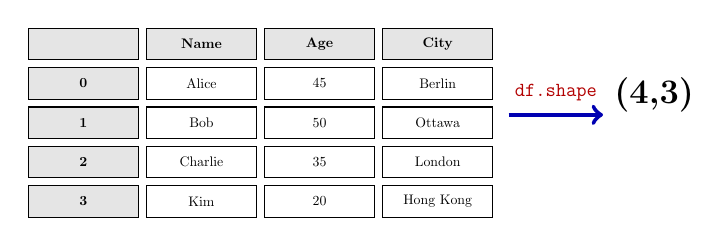
\begin{tikzpicture}[scale=0.5, transform shape,
    cell/.style={
        draw,
        minimum width=2.8cm,
        minimum height=0.8cm,
        align=center
    },
    header/.style={
        cell,
        fill=gray!20,
        font=\bfseries
    }
]

%%%%%%%%%%%%%%%%%%%%%%%%
% DataFrame original
%%%%%%%%%%%%%%%%%%%%%%%%

% --- Headers ---
\node[header] at (0,0) {};
\node[header] at (3,0) {Name};
\node[header] at (6,0) {Age};
\node[header] at (9,0) {City};

% --- Row 0 ---
\node[header] at (0,-1) {0};
\node[cell] at (3,-1) {Alice};
\node[cell] at (6,-1) {45};
\node[cell] at (9,-1) {Berlin};

% --- Row 1 ---
\node[header] at (0,-2) {1};
\node[cell] at (3,-2) {Bob};
\node[cell] at (6,-2) {50};
\node[cell] at (9,-2) {Ottawa};

% --- Row 2 ---
\node[header] at (0,-3) {2};
\node[cell] at (3,-3) {Charlie};
\node[cell] at (6,-3) {35};
\node[cell] at (9,-3) {London};

% --- Row 3 ---
\node[header] at (0,-4) {3};
\node[cell] at (3,-4) {Kim};
\node[cell] at (6,-4) {20};
\node[cell] at (9,-4) {Hong Kong};

%%%%%%%%%%%%%%%%%%%%%%%%
% Flecha df.iloc[0]
%%%%%%%%%%%%%%%%%%%%%%%%

\draw[->, ultra thick, blue!70!black]
    (10.8,-1.8)
    to[out=0,in=180]
    node[midway, above=6pt,
          font=\ttfamily\Large,
          text=red!70!black]
    {df.shape}
    (13.2,-1.8);

%%%%%%%%%%%%%%%%%%%%%%%%
% Resultado df.iloc[0] como Series
%%%%%%%%%%%%%%%%%%%%%%%%

% Título
\node[font=\bfseries\Huge] at (14.5,-1.3) { (4,3) };

%\node[font=\ttfamily\small] at (19.5,-4.2) {Name: 0};

\end{tikzpicture}

        \end{figure}
    \end{frame}


    \begin{frame}[fragile]{Función \mintinline{python}{len}}
        \begin{itemize}
            \item \mintinline{python}{len(df)} devuelve el largo del \emph{DataFrame} medido en número de filas.
        \end{itemize}
        \begin{figure}[H]
            \centering
            \input{len}
        \end{figure}

    \end{frame}

    \begin{frame}[fragile]{Método \mintinline{python}{iloc}}
        \begin{itemize}
            \item \mintinline{python}{df.iloc(k)} devuelve un objeto del tipo \mintinline{python}{pd.Series} generado con la fila en la posición $k$. Si lo viéramos como una lista, acá lo que importa es la posición entera (que ya sabemos, parte de $0$).
        \end{itemize}

        \begin{figure}
            \centering
            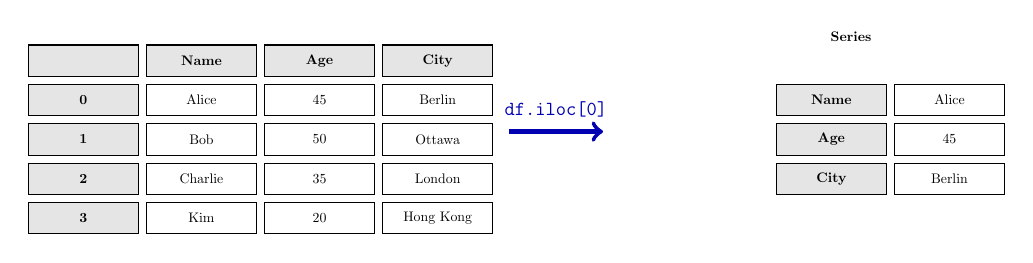
\begin{tikzpicture}[scale=0.5, transform shape,
    cell/.style={
        draw,
        minimum width=2.8cm,
        minimum height=0.8cm,
        align=center
    },
    header/.style={
        cell,
        fill=gray!20,
        font=\bfseries
    }
]

%%%%%%%%%%%%%%%%%%%%%%%%
% DataFrame original
%%%%%%%%%%%%%%%%%%%%%%%%

% --- Headers ---
\node[header] at (0,0) {};
\node[header] at (3,0) {Name};
\node[header] at (6,0) {Age};
\node[header] at (9,0) {City};

% --- Row 0 ---
\node[header] at (0,-1) {0};
\node[cell] at (3,-1) {Alice};
\node[cell] at (6,-1) {45};
\node[cell] at (9,-1) {Berlin};

% --- Row 1 ---
\node[header] at (0,-2) {1};
\node[cell] at (3,-2) {Bob};
\node[cell] at (6,-2) {50};
\node[cell] at (9,-2) {Ottawa};

% --- Row 2 ---
\node[header] at (0,-3) {2};
\node[cell] at (3,-3) {Charlie};
\node[cell] at (6,-3) {35};
\node[cell] at (9,-3) {London};

% --- Row 3 ---
\node[header] at (0,-4) {3};
\node[cell] at (3,-4) {Kim};
\node[cell] at (6,-4) {20};
\node[cell] at (9,-4) {Hong Kong};

%%%%%%%%%%%%%%%%%%%%%%%%
% Flecha df.iloc[0]
%%%%%%%%%%%%%%%%%%%%%%%%

\draw[->, ultra thick, blue!70!black]
    (10.8,-1.8)
    to[out=0,in=180]
    node[midway, above=6pt,
          font=\ttfamily\Large,
          text=blue!70!black]
    {df.iloc[0]}
    (13.2,-1.8);

%%%%%%%%%%%%%%%%%%%%%%%%
% Resultado df.iloc[0] como Series
%%%%%%%%%%%%%%%%%%%%%%%%

% Título
\node[font=\bfseries] at (19.5,0.6) {Series};

% Celdas de la serie (índice, valor)
\node[header] at (19,-1) {Name};
\node[cell] at (22,-1) {Alice};

\node[header] at (19,-2) {Age};
\node[cell] at (22,-2) {45};

\node[header] at (19,-3) {City};
\node[cell] at (22,-3) {Berlin};

% Nombre del índice
%\node[font=\ttfamily\small] at (19.5,-4.2) {Name: 0};

\end{tikzpicture}

        \end{figure}
    \end{frame}


    \begin{frame}[fragile]{Método \mintinline{python}{loc}}
        \begin{itemize}
            \item \mintinline{python}{df.loc(k)} devuelve un objeto del tipo \mintinline{python}{pd.Series} generado con la fila indexada por el valor $k$. Aquí lo que importa es el valor del índice del \emph{DataFrame} (que puede ser cualquier cosa, no necesariamente números enteros consecutivos).
        \end{itemize}
        \begin{figure}[H]
            \centering
            \input{loc}
        \end{figure}
    \end{frame}

    \begin{frame}[fragile]{Leer una columna específica}
        En Python, podemos acceder a los atributos de objetos usando \texttt{[]} después del objeto.
        \begin{itemize}
            \item \mintinline{python}{df[col]} devuelve un objeto de tipo \mintinline{python}{pd.Series} generado con la columna \texttt{col}.
            \item También podemos usar \mintinline{python}{df[["col1", "col2"]]} para obtener varias columnas a la vez (en este caso, \texttt{col1} y \texttt{col2}).
        \end{itemize}
        \begin{figure}[H]
            \centering
            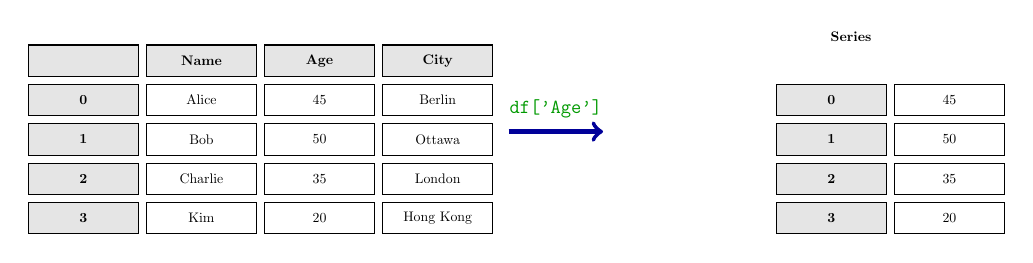
\begin{tikzpicture}[
    scale=0.5, 
    transform shape,
    cell/.style={
        draw,
        minimum width=2.8cm,
        minimum height=0.8cm,
        align=center
    },
    header/.style={
        cell,
        fill=gray!20,
        font=\bfseries
    }
]
    % --- Headers ---
    \node[header] at (0,0) {};
    \node[header] at (3,0) {Name};
    \node[header] at (6,0) {Age};
    \node[header] at (9,0) {City};

    % --- Row 0 ---
    \node[header] at (0,-1) {0};
    \node[cell] at (3,-1) {Alice};
    \node[cell] at (6,-1) {45};
    \node[cell] at (9,-1) {Berlin};

    % --- Row 1 ---
    \node[header] at (0,-2) {1};
    \node[cell] at (3,-2) {Bob};
    \node[cell] at (6,-2) {50};
    \node[cell] at (9,-2) {Ottawa};

    % --- Row 2 ---
    \node[header] at (0,-3) {2};
    \node[cell] at (3,-3) {Charlie};
    \node[cell] at (6,-3) {35};
    \node[cell] at (9,-3) {London};

    % --- Row 3 ---
    \node[header] at (0,-4) {3};
    \node[cell] at (3,-4) {Kim};
    \node[cell] at (6,-4) {20};
    \node[cell] at (9,-4) {Hong Kong};


    \draw[->, ultra thick, blue!60!black]
        (10.8,-1.8)
        to[out=0,in=180]
        node[midway, above=6pt,
            font=\ttfamily\Large,
            text=green!60!black]
        {df['Age']}
        (13.2,-1.8);

    % Title
    \node[font=\bfseries] at (19.5,0.6) {Series};

    % Series cells
    \node[header] at (19,-1) {0};
    \node[cell] at (22,-1) {45};

    \node[header] at (19,-2) {1};
    \node[cell] at (22,-2) {50};

    \node[header] at (19,-3) {2};
    \node[cell] at (22,-3) {35};

    \node[header] at (19,-4) {3};
    \node[cell] at (22,-4) {20};
\end{tikzpicture}

        \end{figure}
    \end{frame}

    \begin{frame}{Resumen de \emph{DataFrames} en \texttt{pandas}}
        \begin{itemize}
            \item \mintinline{python}{df.read_csv()} para cargar un conjunto de datos desde un archivo \texttt{.csv}.
            \item \mintinline{python}{df.head()} para mirar las primeras filas.
            \item \mintinline{python}{df.tail()} para mirar las últimas filas.
            \item \mintinline{python}{df.shape} para obtener las dimensiones de la tabla.
            \item \mintinline{python}{len(df)} para obtener el número de filas en la tabla.
            \item \mintinline{python}{df.columns} para obtener los nombres de las columnas en la tabla.
            \item \mintinline{python}{df.iloc[k]} para obtener la fila ubicada en la posición entera $k$.
            \item \mintinline{python}{df.loc[index]} para obtener la fila asignada al indice \texttt{index}.
            \item \mintinline{python}{df.to_csv()} para guardar el \emph{DataFrame} en un archivo \texttt{.csv}.
        \end{itemize}
        \textbf{Sin embargo, ¡\texttt{pandas} tiene más funciones! Veremos esto mañana...}.
    \end{frame}


    \begin{frame}{\emph{DataFrames} a partir de conjuntos de datos reales}
        En los ejemplos anteriores, generamos \emph{series} y \emph{DataFrames} usando datos creados de manera manual. Sin embargo, en proyectos reales debemos cargar datos desde archivos o páginas web. Esto se puede realizar con las siguientes funciones (Tabla \ref{tab:read_data}).
        \begin{table}[H]
            \centering
            \begin{tabular}{c|p{6cm}|p{5cm}}
                \hline
                \textbf{Función} & \textbf{Uso} & \textbf{Ejemplo} \\
                \hline

                \multirow{2}{*}{\mintinline{python}{read_csv}}
                & \multirow{2}{6cm}{Cargar datos delimitados por comas desde un archivo local o una URL}
                & \multirow{2}{*}{\mintinline{python}{pd.read_csv("datos.csv")}}  \\
                &  \\
                \hline

                \multirow{2}{*}{\mintinline{python}{read_excel}}
                & \multirow{2}{6cm}{Cargar datos tabulares desde un archivo Excel}
                & \multirow{2}{*}{\mintinline{python}{pd.read_excel("datos.xlsx")}} \\
                &  \\
                \hline

                \multirow{2}{*}{\mintinline{python}{read_pickle}}
                & \multirow{2}{6cm}{Cargar datos serializados en formato pickle}
                & \multirow{2}{*}{\mintinline{python}{pd.read_pickle("datos.pkl")}} \\
                &  \\
                \hline

                \multirow{2}{*}{\mintinline{python}{read_json}}
                & \multirow{2}{6cm}{Cargar datos desde archivos JSON}
                & \multirow{2}{*}{\mintinline{python}{pd.read_json("datos.json")}} \\
                &  \\
                \hline
            \end{tabular}
            \caption{Funciones de \texttt{pandas} para carga de datos.}
            \label{tab:read_data}
        \end{table}
    \end{frame}

    \begin{frame}{¿Cómo guardar datos con \texttt{pandas}?}
        Lo último que vamos a ver es cómo guardar un objeto de tipo \mintinline{python}{pd.DataFrame}. Podemos guardarlo usando las siguientes funciones (Tabla \ref{tab:save_data}).

        \begin{table}[h]
            \centering
            \begin{tabular}{c|p{6cm}|p{5cm}}
                \hline
                \textbf{Función} & \textbf{Uso} & \textbf{Ejemplo} \\
                \hline

                \multirow{2}{*}{\mintinline{python}{to_csv}}
                & \multirow{2}{6cm}{Guardar un \emph{DataFrame} en un archivo delimitado por comas (CSV)}
                & \multirow{2}{*}{\mintinline{python}{df.to_csv("datos.csv")}} \\
                &  \\
                \hline

                \multirow{2}{*}{\mintinline{python}{to_excel}}
                & \multirow{2}{6cm}{Guardar un \emph{DataFrame} en un archivo Excel}
                & \multirow{2}{*}{\mintinline{python}{df.to_excel("datos.xlsx")}} \\
                &  \\
                \hline

                \multirow{2}{*}{\mintinline{python}{to_pickle}}
                & \multirow{2}{6cm}{Serializar y guardar un \emph{DataFrame} en formato pickle}
                & \multirow{2}{*}{\mintinline{python}{df.to_pickle("datos.pkl")}} \\
                &  \\
                \hline

                \multirow{2}{*}{\mintinline{python}{to_json}}
                & \multirow{2}{6cm}{Guardar un \emph{DataFrame} en un archivo JSON}
                & \multirow{2}{*}{\mintinline{python}{df.to_json("datos.json")}} \\
                &  \\
                \hline
            \end{tabular}
            \caption{Funciones de \texttt{pandas} para guardar datos.}
            \label{tab:save_data}
        \end{table}
    \end{frame}

    \begin{frame}{Ejemplo práctico}
        Exploraremos un conjunto de datos que tiene información sobre Pokémon en \href{https://colab.research.google.com/drive/1X7xoTisfFrGZFfrQ9ROckTaYzv8Xw8TB?usp=sharing}{Google Colab}, para aplicar lo aprendido en esta clase.
        \begin{figure}[H]
            \centering
            \includegraphics[width=0.5\linewidth]{days/03/images/pokemon.png}
        \end{figure}
    \end{frame}
\end{document}